\documentclass{article}
\usepackage{amsmath}
\usepackage{breqn}
\usepackage{color}
\usepackage{hyperref}
\usepackage{datetime}
\usepackage{graphicx}

\definecolor{heavyblue}{cmyk}{1,1,0,0.25}

\newcommand{\thetitle}{SEME 2016: OptionWay Project Report}
\newcommand{\theauthors}{Malcolm Roberts, Matteo Aletti, Athmane Bakhta, Boris Nectoux}

\title{\thetitle{}}
\author{\theauthors{}}

\hypersetup{
  pdftitle={\thetitle},
  pdfpagemode=UseOutlines,
  citebordercolor=0 0 1,
  colorlinks=true,
  allcolors=heavyblue,
  breaklinks=true,
  pdfauthor={\theauthors},
  pdfpagetransition=Dissolve,
  bookmarks=true
}

% Specify ISO date format:
\yyyymmdddate
\renewcommand{\dateseparator}{-}

\def\abs#1{{\left|#1\right|}}
\def\(#1\){{\left(#1\right)}}
\def\nobr#1{\hiderel{#1}}

\def\aow{\alpha_{\rm{OW}}}
\def\aobs{\alpha_{\rm{obs}}}

\begin{document}

\maketitle

\begin{abstract}
  asdfasdfasdf FIXME
\end{abstract}

\section{Introduction}

Travellers wishing to purchase a flight for a specific day to a
particular destination are faced with a problem: how can they find the
cheapest flight which matches their criteria?  Since the advent of
online travel agents, it is easy to find the cheapest price available
that day, and multiple services are available.  The travel agent
offers a variety of prices from multiple airlines, and the consumer is
free to choose whether or not they wish to buy.  At this point one
would think that the problem is solved, but one must remember that
there is another player in this particular economic game: the airline,
which seeks to sell seats on planes in order to maximize its own
profit.

In general, there are several airlines which compete on a particular
route, such as Paris--New York, and the airlines will vary their prices
according to their own individual strategies (strategies which, we add
parenthetically, produce seemingly bizarre prices).  The airlines
compete with each other, but they can also increase their profit by
adopting a strategy which increases the likelihood that an individual
consumer will purchase a ticket.  In addition, there are circumstances
where a consumer has very low price sensitivity, so it might be good
to occasionally offer higher prices in case such a client is looking
for a flight at the same moment when the high prices are in effect.

The effect of this on the consumer is that there is a significant
amount of variance in the price of the cheapest flight available.  If
the Paris--New York flight is \$1000 today, it might be \$900 next
week, or perhaps \$1100.  Thus the optimal strategy for the consumer
is to check the cost each day to determine the range of prices
available and then to use that information in order to try and get a
better price.  Each day the traveller will visit various websites,
collect data, and, when they think that they have enough information,
start looking for a flight.  While there may certainly be some
travellers who find this sort of activity a great way to spend a
Friday night, the vast majority will probably find the use of their
time sub-optimal for what may end up being a fairly minimal savings in
cost.

The online travel agent OptionWay autmoates this process; the
traveller specifies their destination and travel dates, the price that
they are willing to pay for the trip, and the length of time that they
want OptionWay to look for the ticket.  If their criteria are
satisfied during this time, OptionWay automatically buys the ticket
when the specified price is available.  Using this method, the
traveller is saved the drudgery of manually searching for flights on a
daily basis.

However, the demand price may or may not be likely to appear in the
specified search period.  For example, if the traveller wants to fly
Paris--New York for \$400, they are likley to never find a ticket at
such a price.  OptionWay would like to provide an estimate for the
probability of the chance of success of their demand.

\section{Data and Analysis}

OptionWay provided us with sample data for flights to various
destinations.  The data was composed of all the flight prices for a
particular route for travel on a variety of dates, with flight prices
available from 130 days before the flight to the day of.  Data was not
necessarily available for each day.  There were 12 routes available.
Data was given in the form of csv files, which ranged in size from 13M
to 2.3G. We show a sample of such data in
Figure~\ref{PARFCO_SAT_7_nonorm} for flights between Paris and Rome
from Saturday to Saturday.  In Figure~\ref{PARRUN_SAT_7_nonorm}, we
show data for Paris--Ile Réunion, also for a Saturday-to-Saturday
trip.  While both show a large amount of variance, the Paris-Rome trip
shows a stronger tendency for the price to rise nearer the travel date
than the Paris--Réunion trip.  

%FIXME: we created a python script which deals with this kind of
%thing.

\begin{figure}
  \begin{center}
    % ./plots.py -f data/PARFCO_SAT_7.csv -d PARFCO_SAT_7_nonorm
    % asy datagraphs -u "ymax=500"
    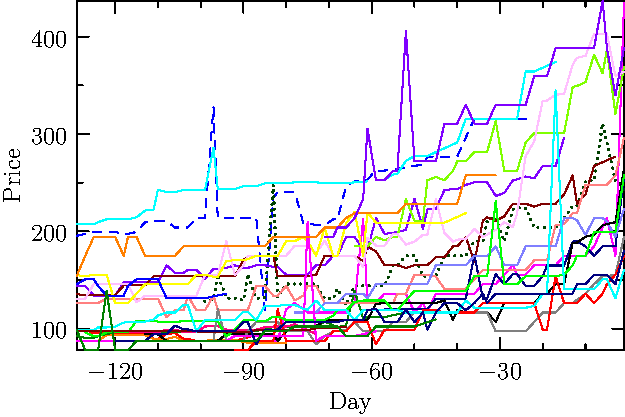
\includegraphics{pdf/PARFCO_SAT_7_nonorm}
    \label{PARFCO_SAT_7_nonorm}
    \caption{Minimum available price as a function of number of days
      before the lgiths for PAR--FCO from Saturday to Saturday for a
      variety of departure dates. Prices abore 500 were excluded.}
  \end{center}
\end{figure}

\begin{figure}
  \begin{center}
    %  ./plots.py -f data/PARRUN_SAT_7.csv -d PARRUN_SAT_7_nonorm
    % asy datagraphs -u "ymax=3000"
    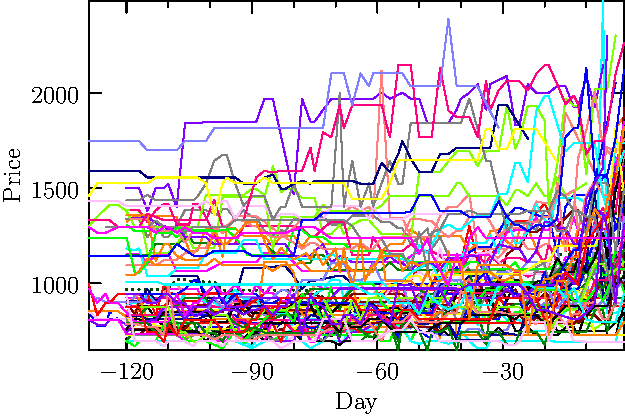
\includegraphics{pdf/PARRUN_SAT_7_nonorm}
    \label{PARRUN_SAT_7_nonorm}
    \caption{Minimum available price as a function of number of days
      before the lgiths for PAR--RUN from Saturday to Saturday for a
      variety of departure dates. Prices abore 3000 were excluded.}
  \end{center}
\end{figure}

\section{Probability Estimators}
The probability of an asking price $p_d$ being achieved during a
search interval $T$ is denoted by $\alpha$.  Let $p(t)$ denote the
minimum price at time $t$, in days, for the a given flight, and $t_0$
the time when the traveller starts looking for a ticket.  As a rough
estimate, OptionWay uses the following formula to predict the
probability that the client will succeed:
\begin{dmath}
  \alpha_{\rm{OW}}(t_o,T,p_d) = \frac{1}{1 + \frac{4500 p(t_0)}{4.5 T}e^{-11 p_d / p(t_0)}}.
  \label{owalpha}
\end{dmath}
The motivation behind this formula was to construct a function that
gives a higher probability when $p_d$ and $T$ are large.

We can test the accuracy of equation~\eqref{owalpha} agains the given
data.  In Figure~\ref{PARRUN_SAT_7_a0}, we show the a colourmap of the
probability of successfully finding a flight at a price $p_d$ for
$t_0=30$.  Notably, there is a large increase in probability in about
30 days before travelling.  We can compare the obsered probability,
$\alpha_{\rm{obs}}$ against equation~\eqref{owalpha} for individual
lines.  Such a comparison is shown in Figure~\ref{PARRUN_SAT_7_a1_A0},
which shows $\alpha_{\rm{obs}}-\alpha_{\rm{OW}}$.  The difference is
almost entirely negative, indicating that the OptionWay estimate errs
heavily on the side of optimism.  
\begin{figure}
  \begin{center}
    %./test.py -f data/PARRUN_SAT_7.csv -a0
    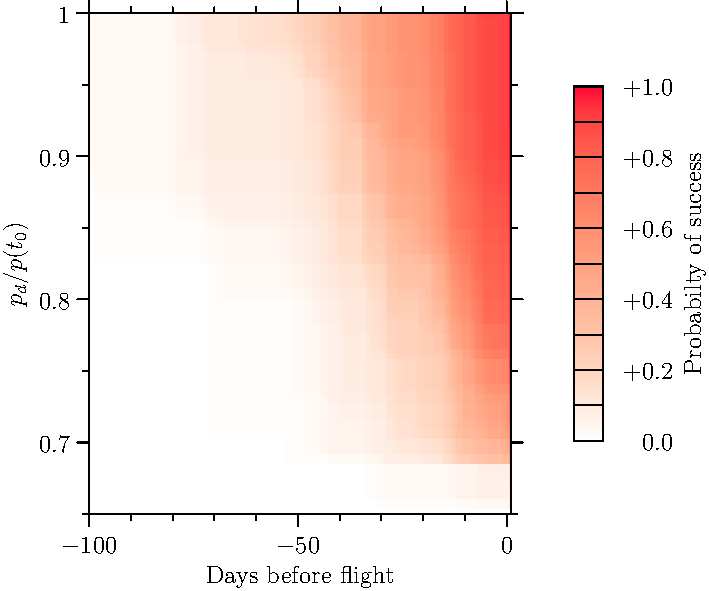
\includegraphics{pdf/PARRUN_SAT_7_a0}
    \label{PARRUN_SAT_7_a0}
    \caption{Probability of success $\alpha_{\rm{obs}}$ for an asking
      price $p_d$ for PAR--RUN for $t_0=30$.}
  \end{center}
\end{figure}
\begin{figure}
  \begin{center}
    %./test.py -f data/PARRUN_SAT_7.csv -a1 -A0
    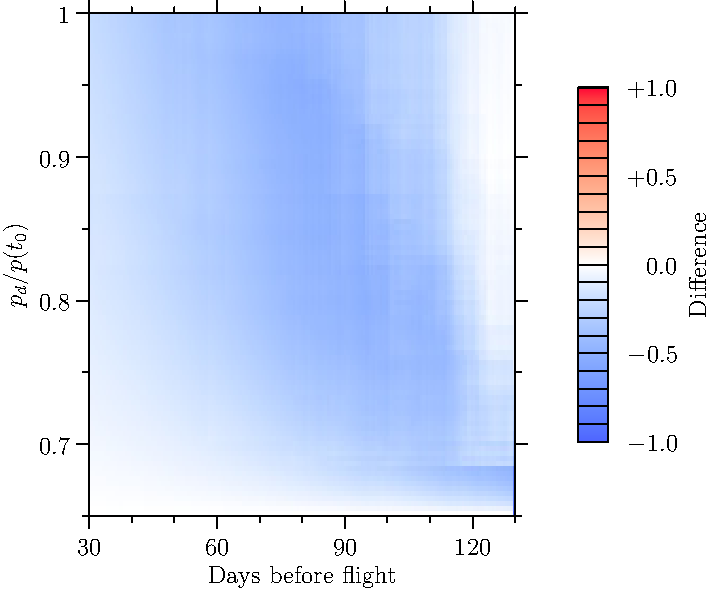
\includegraphics{pdf/PARRUN_SAT_7_a1_A0}
    \label{PARRUN_SAT_7_a1_A0}
    \caption{Difference $\alpha_{\rm{obs}} - \alpha_{\rm{OW}}$ in
      prediction of probability of success between empirical
      measurement and equation~\eqref{owalpha} for an asking price
      $p_d$ for PAR--RUN for $t_0=30$.}
  \end{center}
\end{figure}

In Figure~\ref{plotA0} we show the $L_1$ diference between $\aobs$ and
$\aow$ as a function of $t_0$ for a variety of flights.  For a
majority of the flights considered, $\aow$ has poor accuracy for early
$t_0$, but this improves as the departure date approaches; near the
date of departure, $\aow$ succesfully predicts that a deal is highly
unlikely.  However, there are three cases for which $\aow$ performs
much better.  What is the difference?  Is there some property of these
flights which explains this difference?
\begin{figure}
  \begin{center}
    % ./rundiffA0.sh
    % diff0/PARFCO_MON_123/normvst0.dat,diff0/PARMAD_SAT_7/normvst0.dat,diff0/PARFCO_MON_45/normvst0.dat,diff0/PARNYC_SAT_7/normvst0.dat,diff0/PARFCO_SAT_7/normvst0.dat,diff0/PARRUN_ALL/normvst0.dat,diff0/PARMAD_MON_123/normvst0.dat,diff0/PARRUN_SAT_7/normvst0.dat,diff0/PARMAD_MON_45/normvst0.dat
    %asy datagraphs -u"dolegend=true" -u"legendlist=\"PARFCO_MON_123,PARMAD_SAT_7,PARFCO_MON_45,PARNYC_SAT_7,PARFCO_SAT_7,PARRUN_ALL,PARMAD_MON_123,PARRUN_SAT_7,PARMAD_MON_45\""
    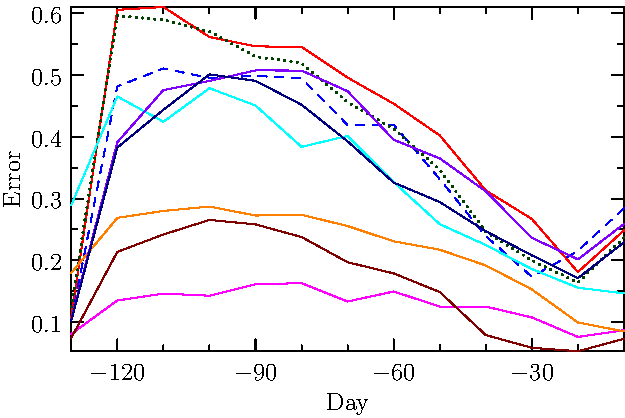
\includegraphics{pdf/plotA0}
    \label{plotA0}
    \caption{Difference between $\alpha_{\rm{OW}}$ and
      $\alpha_{\rm{obs}}$ as a function of $t_0$.}
  \end{center}
\end{figure}

In equation~\eqref{owalpha}, the asking price $p_d$ is divided by the
current minimum price $p(t_0)$.  We can also re-create
figures~\ref{PARFCO_SAT_7_nonorm} and~\ref{PARRUN_SAT_7_nonorm} with
the results scaled by $p(t_0)$.  The results are shown in
Figures~\ref{PARFCO_SAT_7_norm} and~\ref{PARRUN_SAT_7_norm}.  After
normalizing the data, the difference is much more clear; in
Figures~\ref{PARFCO_SAT_7_norm}, there is a strong ris in prices at
around $t_0=-30$, which is much less pronounced in
Figure~\ref{PARRUN_SAT_7_norm}.  The formula given for $\aow$ is
designed to deal with the variance in prices, but neglects any trend.
\begin{figure}
  \begin{center}
    % ./plots.py -f data/PARFCO_SAT_7.csv -d PARFCO_SAT_7_norm -npt0
    % asy datagraphs -u "ymax=2"
    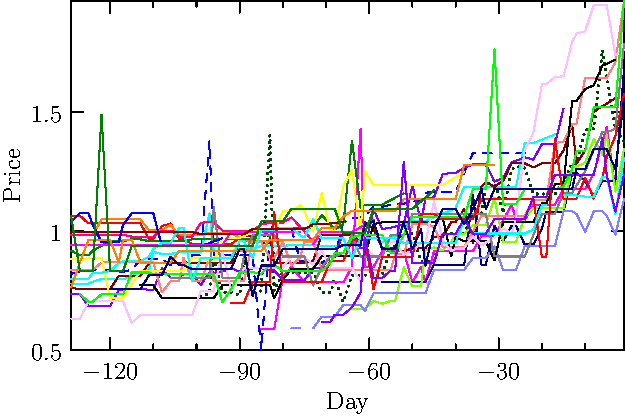
\includegraphics{pdf/PARFCO_SAT_7_norm}
    \label{PARFCO_SAT_7_norm}
    \caption{Minimum available price, normalized by $p(t_0)$, as a
      function of number of days before the lgiths for PAR--FCO from
      Saturday to Saturday for a variety of departure dates. Prices
      with $p_d/p(t_0) > 2$ were excluded.}
  \end{center}
\end{figure}

\begin{figure}
  \begin{center}
    %./plots.py -f data/PARRUN_SAT_7.csv -d PARRUN_SAT_7_norm  -npt0
    % asy datagraphs -u "ymax=2"
    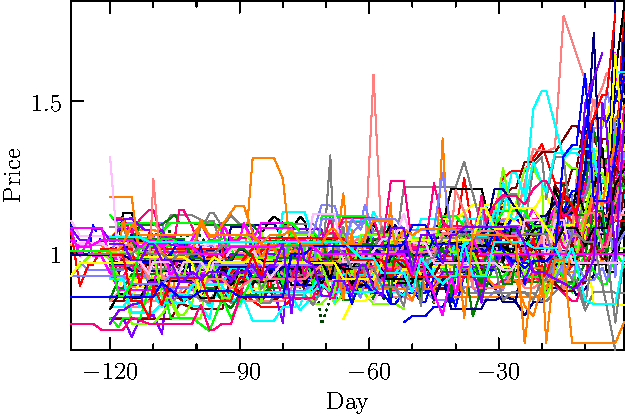
\includegraphics{pdf/PARRUN_SAT_7_norm}
    \label{PARRUN_SAT_7_norm}
    \caption{Minimum available price, normalized by $p(t_0)$, as a
      function of number of days before the lgiths for PAR--RUN from
      Saturday to Saturday for a variety of departure dates.  Prices
      with $p_d/p(t_0) > 2$ were excluded.}
  \end{center}
\end{figure}


FIXME: mention our own hack, say that it might work better.

\section{Conclusion}

FIXME: Summary of what has been done.

FIXME: Future work: look at the distribution.  They are also talking with a
data lab at INRIA who are applying a more statistical model. 

FIXME: Also, look at clustering, particularly so that one can apply
the information to new routes for which one does not yet have a huge
amount of (expensive) data.

FIXME: acknowledgements.

\end{document}
